\chapter{TINJAUAN PUSTAKA}
\vspace{1ex}

\section*{}
Demi mendukung penelitian ini, dibutuhkan beberapa teori penunjang sebagai bahan acuan dan referensi. Dengan demikian penelitian ini menjadi lebih terarah. 
\vspace{1ex}

\section{Jatuh pada Manusia}
\vspace{1ex}

Jatuh adalah kejadian yang tidak disadari dimana seseorang 
terjatuh dari tempat yang lebih tinggi ke tempat yang lebih 
rendah. Banyak sekali penyebab untuk jatuh, salah satunya 
adalah penurunan fisik pada majoritas lanjut usia. 
\vspace{1ex}

\section{Machine Learning}
\vspace{1ex}

Machine Learning (ML) atau Pembelajaran Mesin merupakan bagian 
dari Artificial Intelligence (AI) yang bertujuan untuk memberi 
optimalisasi dalam kriteria dengan cara menganalisa sampel data 
yang terdahulu yang sudah disimpan atau direkam untuk menghasilkan 
sebuah prediksi. Sehingga manusia tidak perlu mengindentifikasi 
sebuah proses sepenuhnya, karena dengan Machine Learning, komputer 
mampu membuat pola untuk membuat keputusan. Machine Learning 
melakukan training yang merupakan proses pembelajaran terhadap 
model data yang sudah terdefinisikan ke beberapa parameter 
(data training) yang menghasilkan beberapa pola sehingga komputer 
dapat melakukan proses klasifikasi berdasarkan pola atau ciri-ciri 
yang sudah didapatkan dalam proses training. Kemudian komputer 
dapat memberikan sebuah prediksi pada data baru selanjutnya 
berdasarkan hasil training. Machine Learning dapat memberi solusi 
dalam berbagai permasalahan seperti Vision (Visi Komputer), Speech 
Recognition (Pengenalan Suara) dan Robotics (Robotika).
\vspace{1ex}

\subsection{\textit{Supervised Learning}}
Desain sistem secara umum pada gambar \ref{fig: 3_1}, yang mencakup disiplin ilmu perangkat keras atau \textit{hardware}, ialah pengolahan citra gambar, visi komputer, sistem tertanam, serta pengolahan sinyal. Disiplin pengolahan citra gambar didapatkan dari pengambilan citra pengemudi menggunakan kamera, visi komputer didapatkan dari proses \textit{recognition} wajah pengemudi, sistem tertanam atau \textit{embedded system} didapatkan dari komunikasi data - data serial menggunakan Arduino atau Mikroprosesor yang tersambung dengan simulator, kemudian yang terakhir Pengolahan sinyal didapatkan dari pengolahan data - data analog seperti data \textit{Electroencephalography (EEG)} / detak jantung pengemudi, atau data \textit{Electrooculography (EOG)} / data kedipan mata dari pengemudi.
\vspace{1ex}

\subsection{\textit{Unsupervised Learning}}
Cakupan Tugas Akhir ini pada bagian perangkat lunak atau \textit{software}, lebih ditekankan dalam upaya pembuatan \textit{Simulation Environment} atau Lingkungan Simulasi menggunakan \textit{Unity Game Engine}. \textit{Simulation Environment} dibuat dengan menggunakan disiplin ilmu grafika komputer 3d (3d \textit{Computer Graphics}), serta juga menggunakan proses - proses pengembangan dari \textit{game engine} dan \textit{physics engine} yang lain.
\vspace{1ex}

\subsection{\textit{Reinforcement Learning}}
\textit{Output} atau keluaran yang diharapkan dari tugas akhir ini ialah, dihasilkannya suatu modul simulasi yang terintegrasi lengkap dengan \textit{tools - tools} dan \textit{peripheral} yang yang dapat mensimulasikan suatu pengalaman mengemudi menggunakan suatu \textit{simulator}, serta dapat melakukan proses pengambilan data - data primer yang valid, sehingga dapat diolah untuk proses riset selanjutnya.
\vspace{1ex}

\section{Deep Learning}
\vspace{1ex}

\begin{figure} [H]
	\captionsetup{justification=centering}
	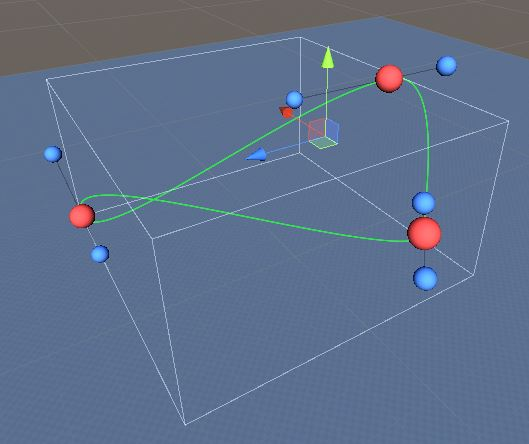
\includegraphics[scale=0.2]{img/contoh-kurva-bezier.JPG}
	\caption{Contoh kurva bezier pada bidang 3 dimensi}
	\label{fig:2.1}
\end{figure}

Deep Learning merupakan artificial neural network yang memiliki banyak layer dan synapse weight. Deep learning dapat menemukan relasi tersembunyi atau pola yang rumit antara input dan
output, yang tidak dapat diselesaikan menggunakan multilayer perceptron (3 layers). Keuntungan utama deep learning yaitu mampu
merubah data dari non-linearly separable menjadi linearly separable
melalui serangkaian transformasi (hidden layers). Selain itu, deep
learning juga mampu mencari decision boundary yang berbentuk
non-linier, serta mengsimulasikan interaksi non-linier antar fitur.
Jadi, input ditransformasikan secara non-linier sampai akhirnya pada output, berbentuk distribusi class-assignment. Pada training
\vspace{1ex}

\section{3D Convolutional Neural Network (3D-CNN)}
\vspace{1ex}

\begin{figure} [H]
	\captionsetup{justification=centering}
	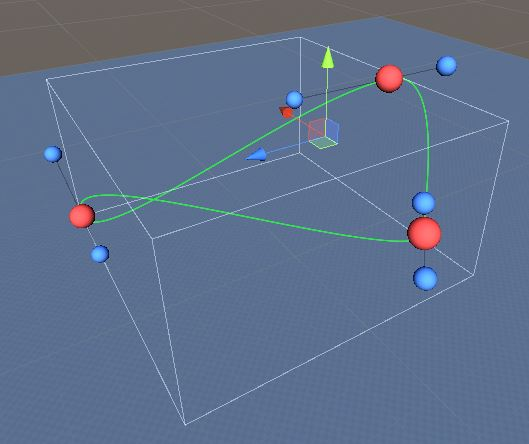
\includegraphics[scale=0.2]{img/contoh-kurva-bezier.JPG}
	\caption{Contoh kurva bezier pada bidang 3 dimensi}
	\label{fig:2.1}
\end{figure}

3D Convolutional Neural Network (CNN) merupakan cabang dari Multilayer Perceptron (MLP) yang digunakan untuk mengolah
data dua dimensi. CNN memiliki kedalaman jaringan yang tinggi
sehingga CNN termasuk dalam jenis Deep Neural Network. Perbedaan CNN dengan MLP terdapat pada neuron dimana pada MLP
setiap neuron hanya berukuran satu dimensi, sedangkan CNN setiap neuronnya berukuran dua dimensi. Pada CNN, operasi linier
menggunakan operasi konvolusi. Bobot pada CNN berbentuk empat dimensi seperti pada Gambar 2.2. Persamaan 2.1 untuk dimensi
bobot pada CNN.
\vspace{1ex}

\subsection{\textit{Convolutional Layer}}
Desain sistem secara umum pada gambar \ref{fig: 3_1}, yang mencakup disiplin ilmu perangkat keras atau \textit{hardware}, ialah pengolahan citra gambar, visi komputer, sistem tertanam, serta pengolahan sinyal. Disiplin pengolahan citra gambar didapatkan dari pengambilan citra pengemudi menggunakan kamera, visi komputer didapatkan dari proses \textit{recognition} wajah pengemudi, sistem tertanam atau \textit{embedded system} didapatkan dari komunikasi data - data serial menggunakan Arduino atau Mikroprosesor yang tersambung dengan simulator, kemudian yang terakhir Pengolahan sinyal didapatkan dari pengolahan data - data analog seperti data \textit{Electroencephalography (EEG)} / detak jantung pengemudi, atau data \textit{Electrooculography (EOG)} / data kedipan mata dari pengemudi.
\vspace{1ex}

\subsection{\textit{Subsampling Layer}}
Cakupan Tugas Akhir ini pada bagian perangkat lunak atau \textit{software}, lebih ditekankan dalam upaya pembuatan \textit{Simulation Environment} atau Lingkungan Simulasi menggunakan \textit{Unity Game Engine}. \textit{Simulation Environment} dibuat dengan menggunakan disiplin ilmu grafika komputer 3d (3d \textit{Computer Graphics}), serta juga menggunakan proses - proses pengembangan dari \textit{game engine} dan \textit{physics engine} yang lain.
\vspace{1ex}

\subsection{\textit{Batch Normalization Layer}}
Cakupan Tugas Akhir ini pada bagian perangkat lunak atau \textit{software}, lebih ditekankan dalam upaya pembuatan \textit{Simulation Environment} atau Lingkungan Simulasi menggunakan \textit{Unity Game Engine}. \textit{Simulation Environment} dibuat dengan menggunakan disiplin ilmu grafika komputer 3d (3d \textit{Computer Graphics}), serta juga menggunakan proses - proses pengembangan dari \textit{game engine} dan \textit{physics engine} yang lain.
\vspace{1ex}

\subsection{\textit{Fully-Connected Layer}}
\textit{Output} atau keluaran yang diharapkan dari tugas akhir ini ialah, dihasilkannya suatu modul simulasi yang terintegrasi lengkap dengan \textit{tools - tools} dan \textit{peripheral} yang yang dapat mensimulasikan suatu pengalaman mengemudi menggunakan suatu \textit{simulator}, serta dapat melakukan proses pengambilan data - data primer yang valid, sehingga dapat diolah untuk proses riset selanjutnya.
\vspace{1ex}

\section{Visi Komputer}
\vspace{1ex}

Visi Komputer adalah cabang Artificial Intelligent (AI) yang
mencakup proses analisa citra dan video. Visi komputer mengimplementasikan beberapa kemampuan visual manusia yang diteruskan
menuju otak seperti deteksi benda, pengenalan wajah dan mengenali bahaya.
Pada visi komputer, Deep Learning sering digunakan untuk pengenalan dan deteksi objek. Proses Deep Learning pada visi komputer memanfaatkan piksel pada citra untuk ekstrasi pola atau atribut
dari citra yang ingin dideteksi. Akan tetapi, hal tersebut mengakibatkan sistem komputasi menjadi lama karena pada suatu citra
mengandung ribuan piksel. Sehingga banyak arsitektur visi komputer membuat standar ukuran, jadi citra tersebut harus dipotong
atau diperkecil untuk mempercepat proses komputasi.
\vspace{1ex}

\section{Image Processing}
\vspace{1ex}

\begin{figure} [H]
	\captionsetup{justification=centering}
	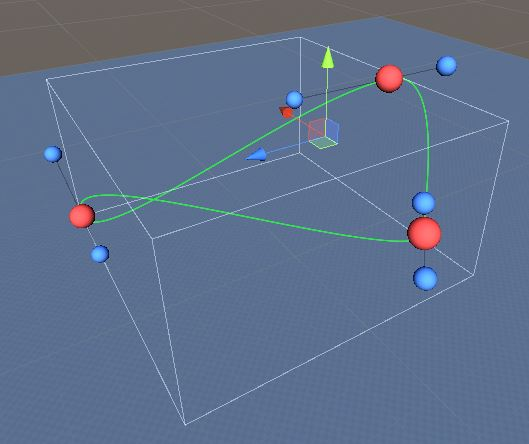
\includegraphics[scale=0.2]{img/contoh-kurva-bezier.JPG}
	\caption{Contoh kurva bezier pada bidang 3 dimensi}
	\label{fig:2.1}
\end{figure}

Image Processing atau Pengolahan Citra merupakan teknik
dalam pemrosesan gambar dengan input berupa citra dua dimensi yang bertujuan untuk menyempurnakan citra atau mendapatkan
informasi yang berguna untuk diolah menjadi beberapa keputusan. Dalam operasi pemrosesan citra, operasi yang sering dilakukan
dalam gambar grayscale. Gambar grayscale didapatkan dari pemrosesan gambar berwarna yang didekomposisi menjadi komponen
merah (R), hijau (G) dan biru (B) yang diproses secara independen
sebagai gambar grayscale. Image Processing terbagi menjadi dalam
\vspace{1ex}

\section{Sistem Tertanam}
\vspace{1ex}

\begin{figure} [H]
	\captionsetup{justification=centering}
	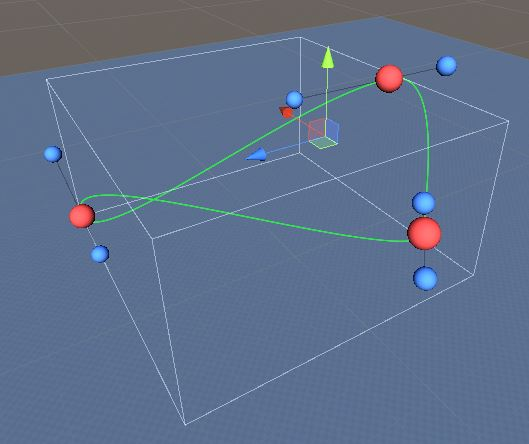
\includegraphics[scale=0.2]{img/contoh-kurva-bezier.JPG}
	\caption{Contoh kurva bezier pada bidang 3 dimensi}
	\label{fig:2.1}
\end{figure}

Image Processing atau Pengolahan Citra merupakan teknik
dalam pemrosesan gambar dengan input berupa citra dua dimensi yang bertujuan untuk menyempurnakan citra atau mendapatkan
informasi yang berguna untuk diolah menjadi beberapa keputusan. Dalam operasi pemrosesan citra, operasi yang sering dilakukan
dalam gambar grayscale. Gambar grayscale didapatkan dari pemrosesan gambar berwarna yang didekomposisi menjadi komponen
merah (R), hijau (G) dan biru (B) yang diproses secara independen
sebagai gambar grayscale. Image Processing terbagi menjadi dalam.
\vspace{1ex}

\section{Metode Pengujian}
\vspace{1ex}

\begin{figure} [H]
	\captionsetup{justification=centering}
	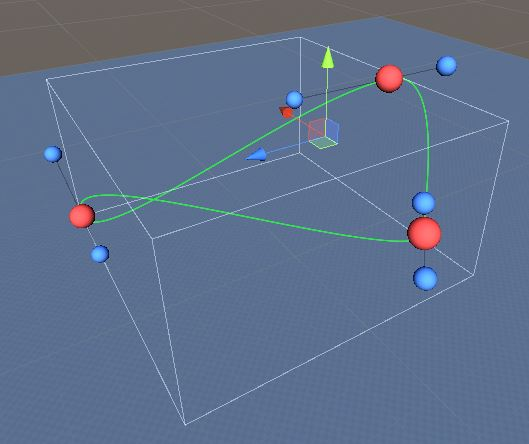
\includegraphics[scale=0.2]{img/contoh-kurva-bezier.JPG}
	\caption{Contoh kurva bezier pada bidang 3 dimensi}
	\label{fig:2.1}
\end{figure}

\textit{3D Convolutional Neural Network} adalah suatu arsitektur neural network dimana mengekstrak fitur dari dimensi spasial dan temporal dengan melakukan konvolusi 3D, sehingga menangkap informasi gerakan yang dikodekan dalam beberapa bingkai yang berdekatan. Arsitektur yang digunakan menghasilkan banyak saluran informasi dari bingkai masukan, dan representasi fitur akhir menggabungkan informasi dari semua saluran.
\vspace{1ex}

\subsection{\textit{Recall}}
Desain sistem secara umum pada gambar \ref{fig: 3_1}, yang mencakup disiplin ilmu perangkat keras atau \textit{hardware}, ialah pengolahan citra gambar, visi komputer, sistem tertanam, serta pengolahan sinyal. Disiplin pengolahan citra gambar didapatkan dari pengambilan citra pengemudi menggunakan kamera, visi komputer didapatkan dari proses \textit{recognition} wajah pengemudi, sistem tertanam atau \textit{embedded system} didapatkan dari komunikasi data - data serial menggunakan Arduino atau Mikroprosesor yang tersambung dengan simulator, kemudian yang terakhir Pengolahan sinyal didapatkan dari pengolahan data - data analog seperti data \textit{Electroencephalography (EEG)} / detak jantung pengemudi, atau data \textit{Electrooculography (EOG)} / data kedipan mata dari pengemudi.
\vspace{1ex}

\subsection{\textit{Precision}}
Cakupan Tugas Akhir ini pada bagian perangkat lunak atau \textit{software}, lebih ditekankan dalam upaya pembuatan \textit{Simulation Environment} atau Lingkungan Simulasi menggunakan \textit{Unity Game Engine}. \textit{Simulation Environment} dibuat dengan menggunakan disiplin ilmu grafika komputer 3d (3d \textit{Computer Graphics}), serta juga menggunakan proses - proses pengembangan dari \textit{game engine} dan \textit{physics engine} yang lain.
\vspace{1ex}

\subsection{\textit{F-Measure}}
Cakupan Tugas Akhir ini pada bagian perangkat lunak atau \textit{software}, lebih ditekankan dalam upaya pembuatan \textit{Simulation Environment} atau Lingkungan Simulasi menggunakan \textit{Unity Game Engine}. \textit{Simulation Environment} dibuat dengan menggunakan disiplin ilmu grafika komputer 3d (3d \textit{Computer Graphics}), serta juga menggunakan proses - proses pengembangan dari \textit{game engine} dan \textit{physics engine} yang lain.
\vspace{1ex}

\subsection{\textit{mean Average Precision (mAP)}}
\textit{Output} atau keluaran yang diharapkan dari tugas akhir ini ialah, dihasilkannya suatu modul simulasi yang terintegrasi lengkap dengan \textit{tools - tools} dan \textit{peripheral} yang yang dapat mensimulasikan suatu pengalaman mengemudi menggunakan suatu \textit{simulator}, serta dapat melakukan proses pengambilan data - data primer yang valid, sehingga dapat diolah untuk proses riset selanjutnya.
\vspace{1ex}

\subsection{\textit{Confusion Matrix}}
\textit{Output} atau keluaran yang diharapkan dari tugas akhir ini ialah, dihasilkannya suatu modul simulasi yang terintegrasi lengkap dengan \textit{tools - tools} dan \textit{peripheral} yang yang dapat mensimulasikan suatu pengalaman mengemudi menggunakan suatu \textit{simulator}, serta dapat melakukan proses pengambilan data - data primer yang valid, sehingga dapat diolah untuk proses riset selanjutnya.
\vspace{1ex}